\chapter{Early Visual System}
\label{chap:visual_system}

In this thesis, we focus on modeling the primary visual cortex (V1), a region that plays a crucial role in early visual processing in the mammalian brain. V1 is among the most studied brain areas and has been a topic of extensive research for decades (\citet{hubel1965receptive}). This chapter highlights the aspects of the visual system that are most relevant to our work. For a more comprehensive overview, we recommend referring to the textbook \citet{bear2020neuroscience} (3rd. Edition) and \citet{goebel2004visual}.

\section{Neuron}
\label{sec:neuron}

The fundamental unit of neural processing is the \emph{neuron}, a specialized cell composed of three primary parts: the soma, the axon, and the dendrites. The soma, or cell body, contains the nucleus and other organelles, and is structurally similar to other cell types. Dendrites are branched extensions that receive signals from other neurons. The axon is a long projection that transmits electrical impulses away from the soma toward other neurons.

\subsection{Axon Overview}
\label{subsec:axon}

The axon originates from the \emph{axon hillock} and terminates at the \emph{axon terminal}, where it forms a \emph{synapse} with the target cell. For efficient signal transmission, the axon contains specialized proteins for propagating electrical potentials. The axon terminal is rich in \emph{synaptic vesicles} containing \emph{neurotransmitters}—chemical messengers such as glutamate, gamma-aminobutyric acid (GABA), glycine, and acetylcholine that facilitate communication between neurons.

A detailed illustration of neuronal anatomy is provided in Figure~\ref{fig:neuron}. Further discussion on neuronal architecture can be found in \citet{bear2020neuroscience} (3rd Edition, p. 28--45).

\begin{figure}
    \centering
    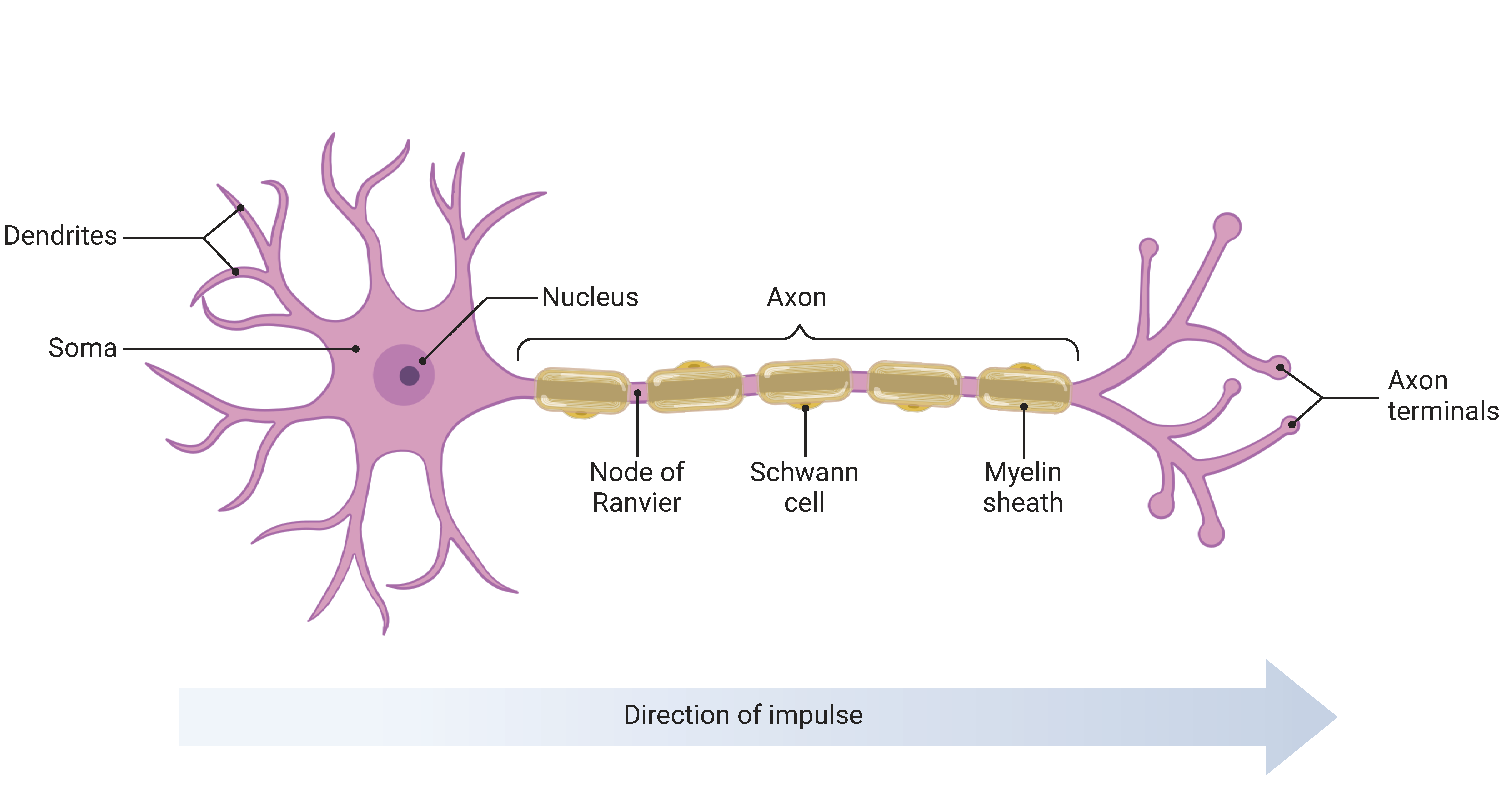
\includegraphics[width=\linewidth]{img/neuron_anatomy.pdf}
    \caption{\textbf{Neuron Anatomy.} A schematic illustration of the structural components of a typical neuron. "Created in BioRender. Beinhauer, D. (2025) https://BioRender.com/m351rlh".}
    \label{fig:neuron}
\end{figure}

\subsection{Action Potential}
\label{subsec:action_potential}

The primary function of neurons is to propagate \emph{action potentials}, enabling communication with other neurons or target cells. This process relies on differences in ion concentrations and electrical potentials across the cell membrane. Key concepts include the \emph{membrane potential}—the voltage difference between the inside and outside of the neuron and \emph{equilibrium potentials}, where electrochemical forces are balanced.

Ion types central to this mechanism include sodium ($\text{Na}^+$), potassium ($\text{K}^+$), chloride ($\text{Cl}^-$), and calcium ($\text{Ca}^{2+}$). All except potassium are typically found in higher concentrations outside the cell. Maintaining these gradients is energetically demanding and accounts for a substantial portion of the brain's energy consumption.

The resting membrane potential of a neuron is approximately $-65$~mV. Action potentials are initiated and propagated along the axonal membrane through the coordinated opening and closing of ion channels. The temporal profile of an action potential is shown in Figure~\ref{fig:action_potential}.

\begin{figure}
    \centering
    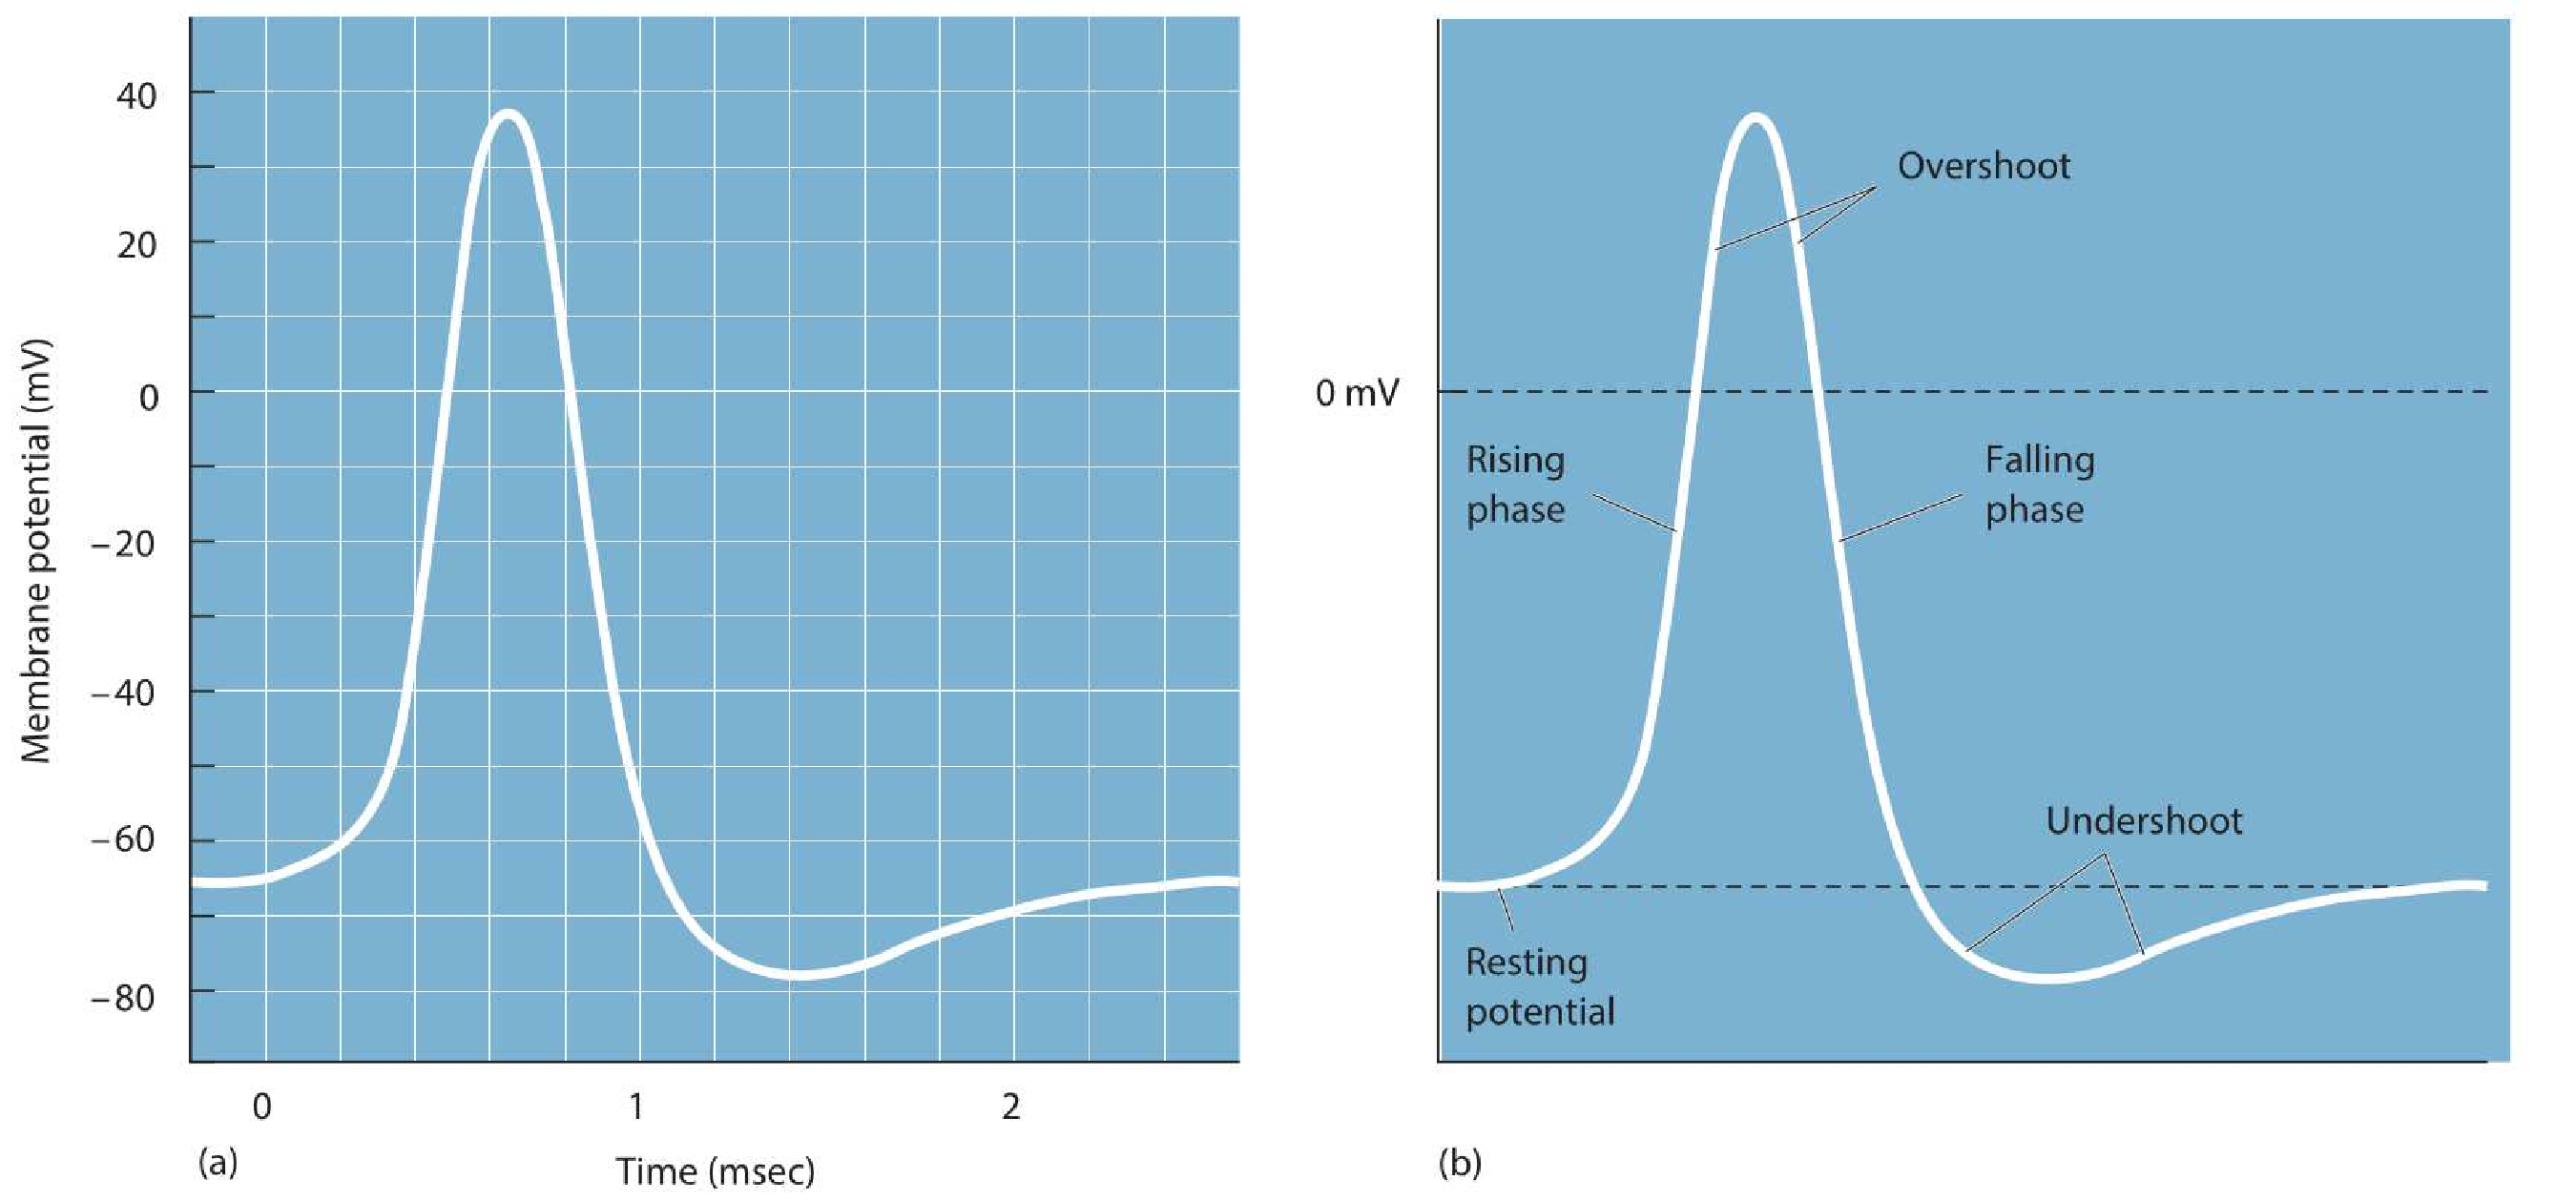
\includegraphics[width=\linewidth]{img/action_potential.pdf}
    \caption{\textbf{An action potential.} \textbf{a)} Oscilloscope trace of an action potential. \textbf{b)} Annotated phases of an action potential. The figure and the labels are taken from \emph{Neuroscience} (\citet{bear2020neuroscience}, 3rd Edition, p. 77).}
    \label{fig:action_potential}
\end{figure}

To accelerate signal conduction over long distances, axons are often insulated by \emph{myelin}, which enables \emph{saltatory conduction} via gaps called \emph{nodes of Ranvier}. This arrangement significantly increases propagation speed. 

For a more detailed understanding of these processes, see \citet{bear2020neuroscience}, 3rd Edition, p. 52--98.

\subsection{Synaptic Transmission}
\label{subsec:synaptic_transmission}

At the synapse, neurotransmitters are released by exocytosis when the action potential reaches the axon terminal. Synaptic connections can be either \emph{excitatory}, leading to membrane depolarization and potential generation of an action potential, or \emph{inhibitory}, which hyperpolarize the target cell and suppress firing.

Additionally, synaptic strength can adapt over short timescales based on recent activity, a phenomenon known as \emph{synaptic depression} (\citet{abbott1997syndepression}). This adaptive behavior is commonly modeled in simulation frameworks and plays a critical role in temporal filtering and network dynamics.

For a more detailed understanding of these processes, see \citet{bear2020neuroscience}, 3rd Edition, p. 102--131.


\section{General Structure of the Early Visual System}
\label{sec:general_structure}

A significant part of the human brain is involved in visual processing. The initial stage of this process occurs within the so-called \emph{early visual system}.

\begin{figure}
    \centering
    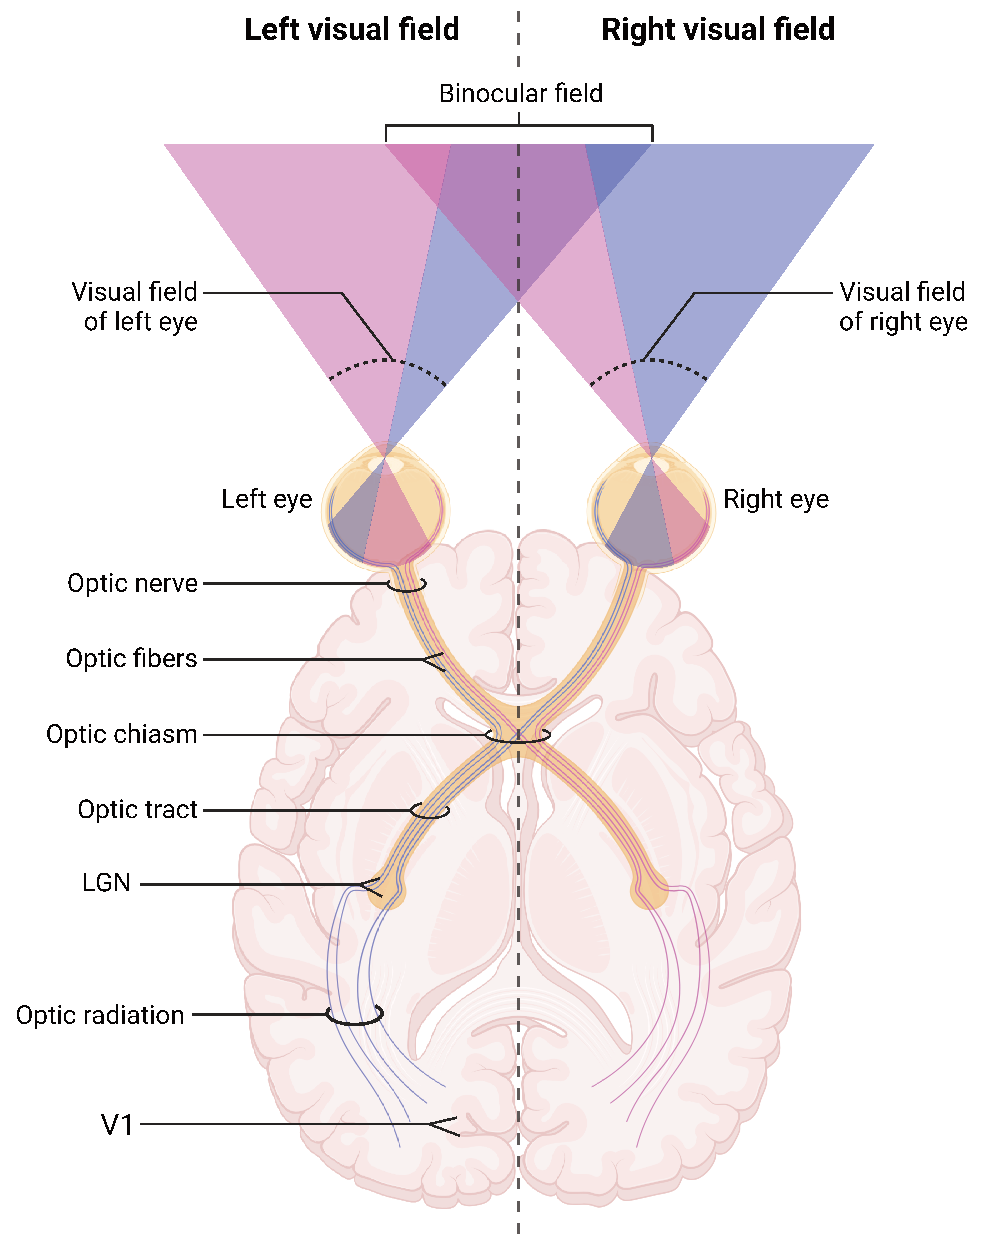
\includegraphics[width=0.6\linewidth]{img/visual_pathway.pdf}
    \caption{\textbf{Anatomical Pathway of Visual Information Processing.} Schematic representation of the anatomical pathway of visual information in the early visual system, tracing the route from the eye to the primary visual cortex. Adapted from \citet{yaramothu2014short} and elaborated with the description from \citet{bear2020neuroscience} (3rd Edition, p. 311--314). "Created in BioRender. Beinhauer, D. (2025) https://BioRender.com/wpfx0a2".}
    \label{fig:visual_system_pathway}
\end{figure}

\begin{figure}
    \centering
    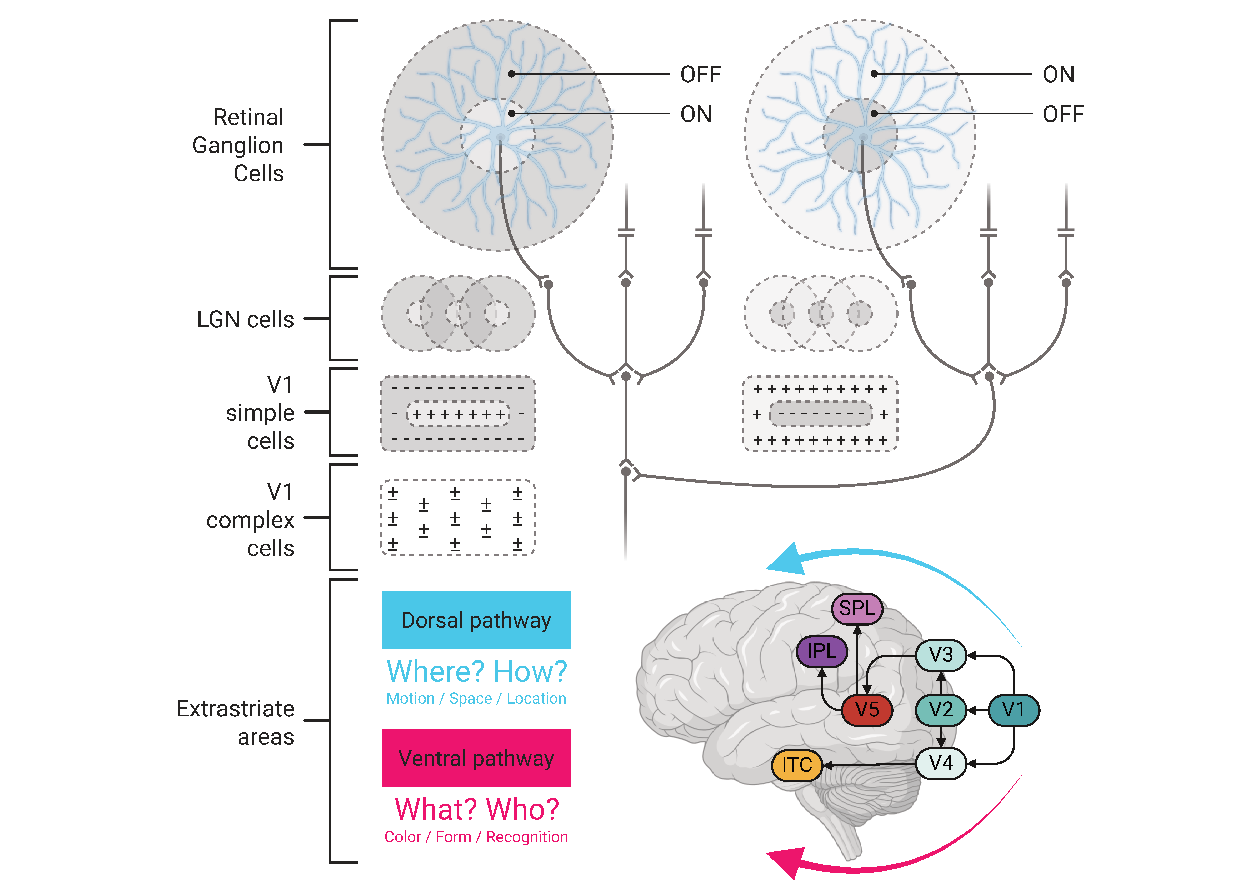
\includegraphics[width=\linewidth]{img/early_visual_processing.pdf}
    \caption{\textbf{Stages of Visual Processing in the Brain.} Schematic depiction of visual information flow from retinal ganglion cells to extrastriate cortical areas. The figure illustrates the receptive fields associated with each stage: starting with ON and OFF retinal ganglion cells and their concentric receptive fields, progressing through LGN cells, and into V1 where simple cells respond to centrally positioned oriented lines and complex cells to oriented lines regardless of exact position. The signal continues to higher-order extrastriate areas involved in advanced visual processing. Adapted from \citet{felleman_distributed_1991} and collaborated with the information from \citet{bear2020neuroscience} (3rd Edition, p. 298--303, 316--337). "Created in BioRender. Beinhauer, D. (2025) https://BioRender.com/byl57wb".}
    \label{fig:early_vis_processing}
\end{figure}

Visual information enters the system in the form of light, which passes through the eye's complex optical apparatus and is projected onto the retina. The retina is a thin layer of neural tissue responsible for detecting light and initiating signal processing. From there, signals travel through the \emph{optic nerve} to the \emph{optic chiasm}, where fibers are sorted based on the visual field, then continue via the \emph{optic tract} to the \emph{lateral geniculate nucleus} (LGN) of the thalamus.

The LGN performs early-stage processing and forwards most of the visual input to the \emph{primary visual cortex} (V1) via the optic radiation. V1 is the first cortical region dedicated to visual analysis, where more complex computations begin. Signals leaving V1 proceed to higher-order visual areas responsible for advanced visual perception. The anatomical pathway from the eye to V1 is depicted in Figure~\ref{fig:visual_system_pathway}, and the transformation of receptive fields throughout visual stages is illustrated in Figure~\ref{fig:early_vis_processing}.

\section{Eye}
\label{sec:eye}

One of the primary roles of the eye is to capture electromagnetic signals from the environment, focus them using its optical system, and project them onto the retina. The eye consists of several specialized structures that modulate and direct light. An anatomical overview is presented in Figure~\ref{fig:eye} and further discussed in \citet{bear2020neuroscience, snell2013clinical}.

\begin{figure}
    \centering
    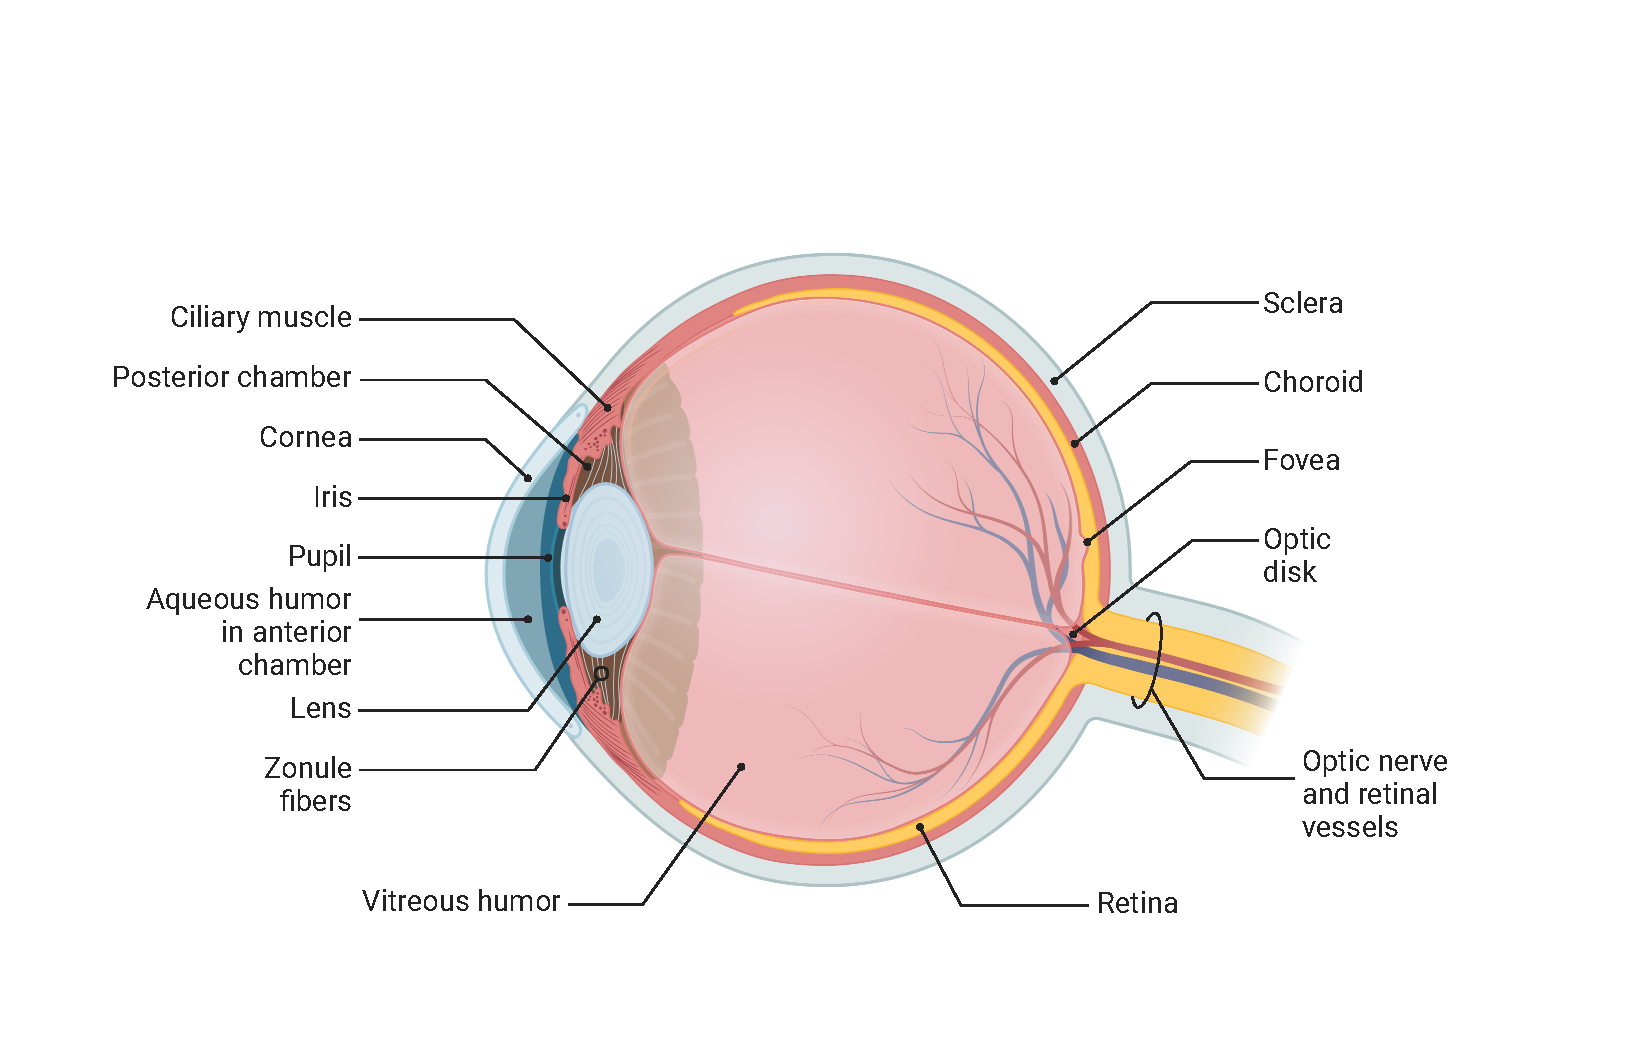
\includegraphics[width=\linewidth]{img/eye.pdf}
    \caption{\textbf{An anatomy of an eye.} Illustration based on (\citet{bear2020neuroscience}, 3rd Edition, p. 283). "Created in BioRender. Beinhauer, D. (2025) https://BioRender.com/8n8epge".}
    \label{fig:eye}
\end{figure}

\subsection{Retina}
\label{subsec:retina}

A second essential function of the eye is the conversion and initial preprocessing of light into neural signals suitable for further brain processing. This task is carried out by the retina—a thin neural tissue layer located at the back of the eye. It is composed of multiple types of cells organized in distinct layers, each contributing to signal modulation. These include photoreceptors, bipolar cells, horizontal cells, amacrine cells, and ganglion cells.

The first cells involved in visual processing are the \emph{photoreceptors}, namely \emph{rods} and \emph{cones}. These cells utilize photochemical reactions in their outer segments to convert light into chemical signals. Rods are highly sensitive to low light and detect a wide range of wavelengths, making them crucial for scotopic (low-light) vision. Cones, by contrast, are less light-sensitive but selective for specific wavelengths and are responsible for color vision and visual acuity.

Photoreceptors are distributed non-uniformly across the retina. The \emph{fovea}, the central region of the retina, is densely packed with cones, while the peripheral retina predominantly contains rods. Additionally, the \emph{optic disc}, or \emph{blind spot}, is a region devoid of photoreceptors where the optic nerve exits the eye.

Upon activation, photoreceptors hyperpolarize and release the neurotransmitter glutamate. This signal is detected by \emph{bipolar cells}, which serve as an intermediary step in the signal pathway. Notably, most retinal cells operate via graded potentials, with the exception of ganglion cells, which fire action potentials (Section~\ref{subsec:action_potential}).

The signal is further processed by \emph{bipolar cells}, which aggregate input from varying numbers of photoreceptors depending on retinal location and cell type. This mechanism emphasizes foveal detail by focusing higher visual resolution centrally. Bipolar cells interact closely with \emph{horizontal cells}, which contribute to lateral inhibition and temporal contrast.

Bipolar, ganglion, and LGN cells are categorized into \emph{ON} and \emph{OFF} types. ON bipolar cells are excited by illumination at the center of their receptive field, whereas OFF cells are excited when the center of receptive field is less illuminated than the surrounding area. This organization is visualized in Figure~\ref{fig:on_off_cells}.

\begin{figure}
    \centering
    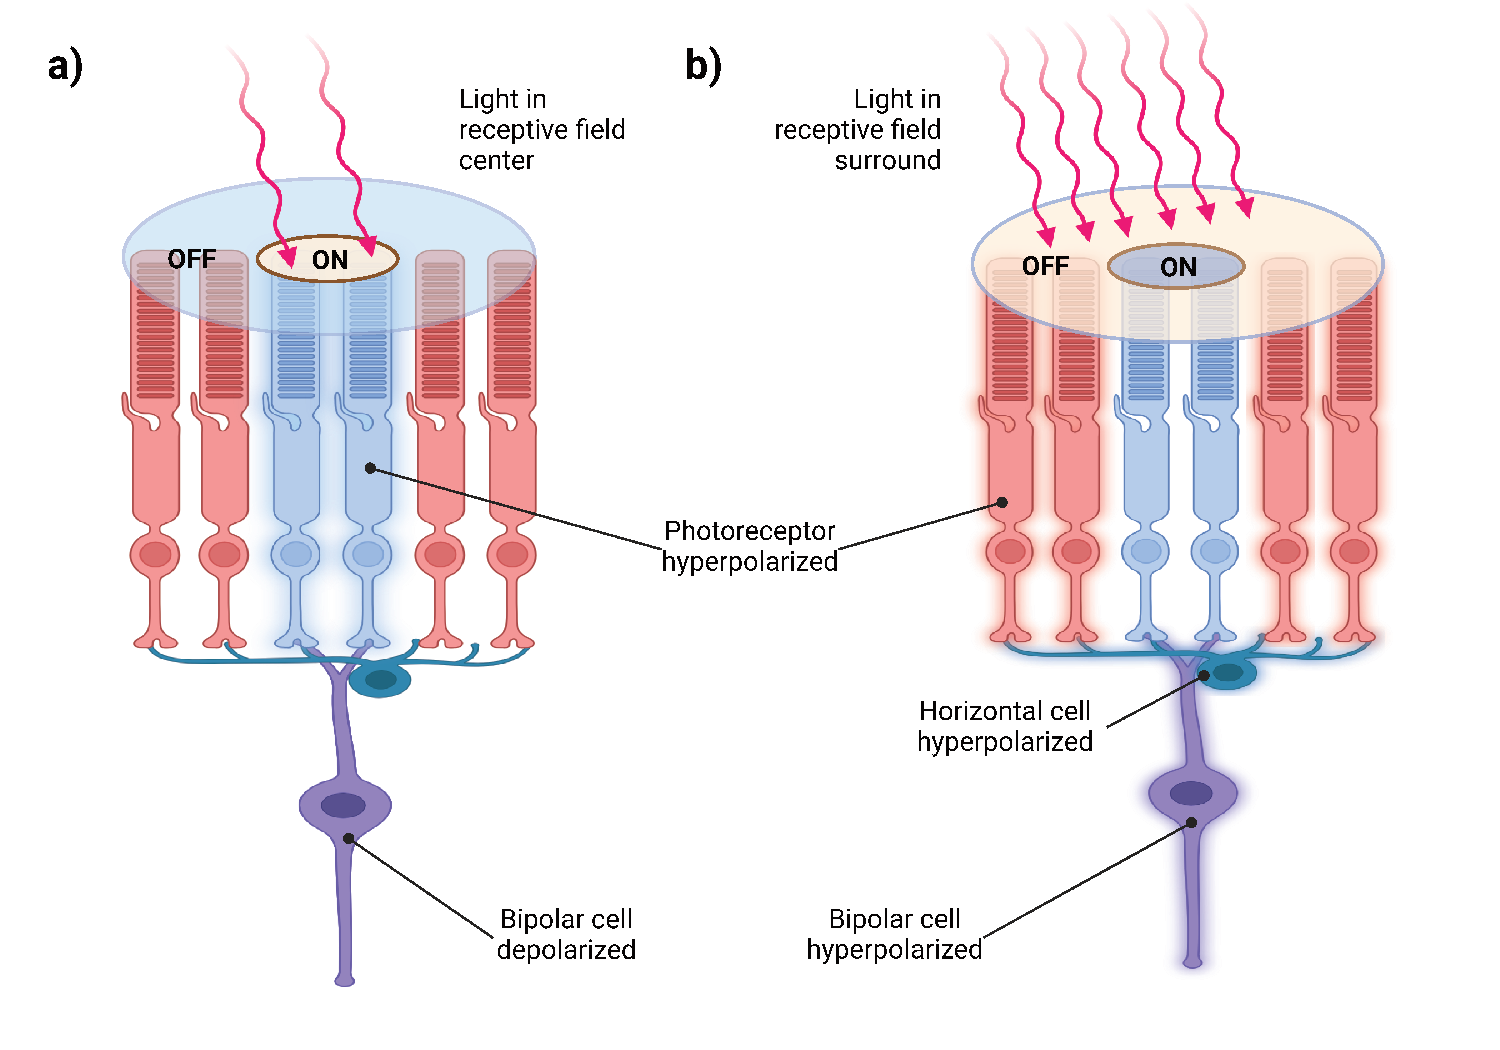
\includegraphics[width=\linewidth]{img/on_off_cells.pdf}
    \caption{\textbf{Direct and indirect pathways from photoreceptors to bipolar cells.} \textbf{a)} An ON bipolar cell depolarizes in response to light in the center of its receptive field. \textbf{b)} The same cell hyperpolarizes in response to surround stimulation. Adapted from \emph{Neuroscience} (\citet{bear2020neuroscience}, 3rd Edition, p. 300). "Created in BioRender. Beinhauer, D. (2025) https://BioRender.com/bpeqbrd".}
    \label{fig:on_off_cells}
\end{figure}

The signal is then transmitted to \emph{ganglion cells}, which interact with \emph{amacrine cells}. Signal processing at this level follows similar principles to those seen in bipolar and horizontal cell interactions. Ganglion cells are the first neurons in the pathway to generate action potentials, which is essential for transmitting signals over long distances to the brain. Their axons converge to form the optic nerve, terminating in the \emph{lateral geniculate nucleus (LGN)} of the thalamus. The retina's layered structure is shown in Figure~\ref{fig:retina_anatomy}. For further details on retinal signal processing, see \citet{bear2020neuroscience} (3rd Edition, p. 288--306).

\begin{figure}
    \centering
    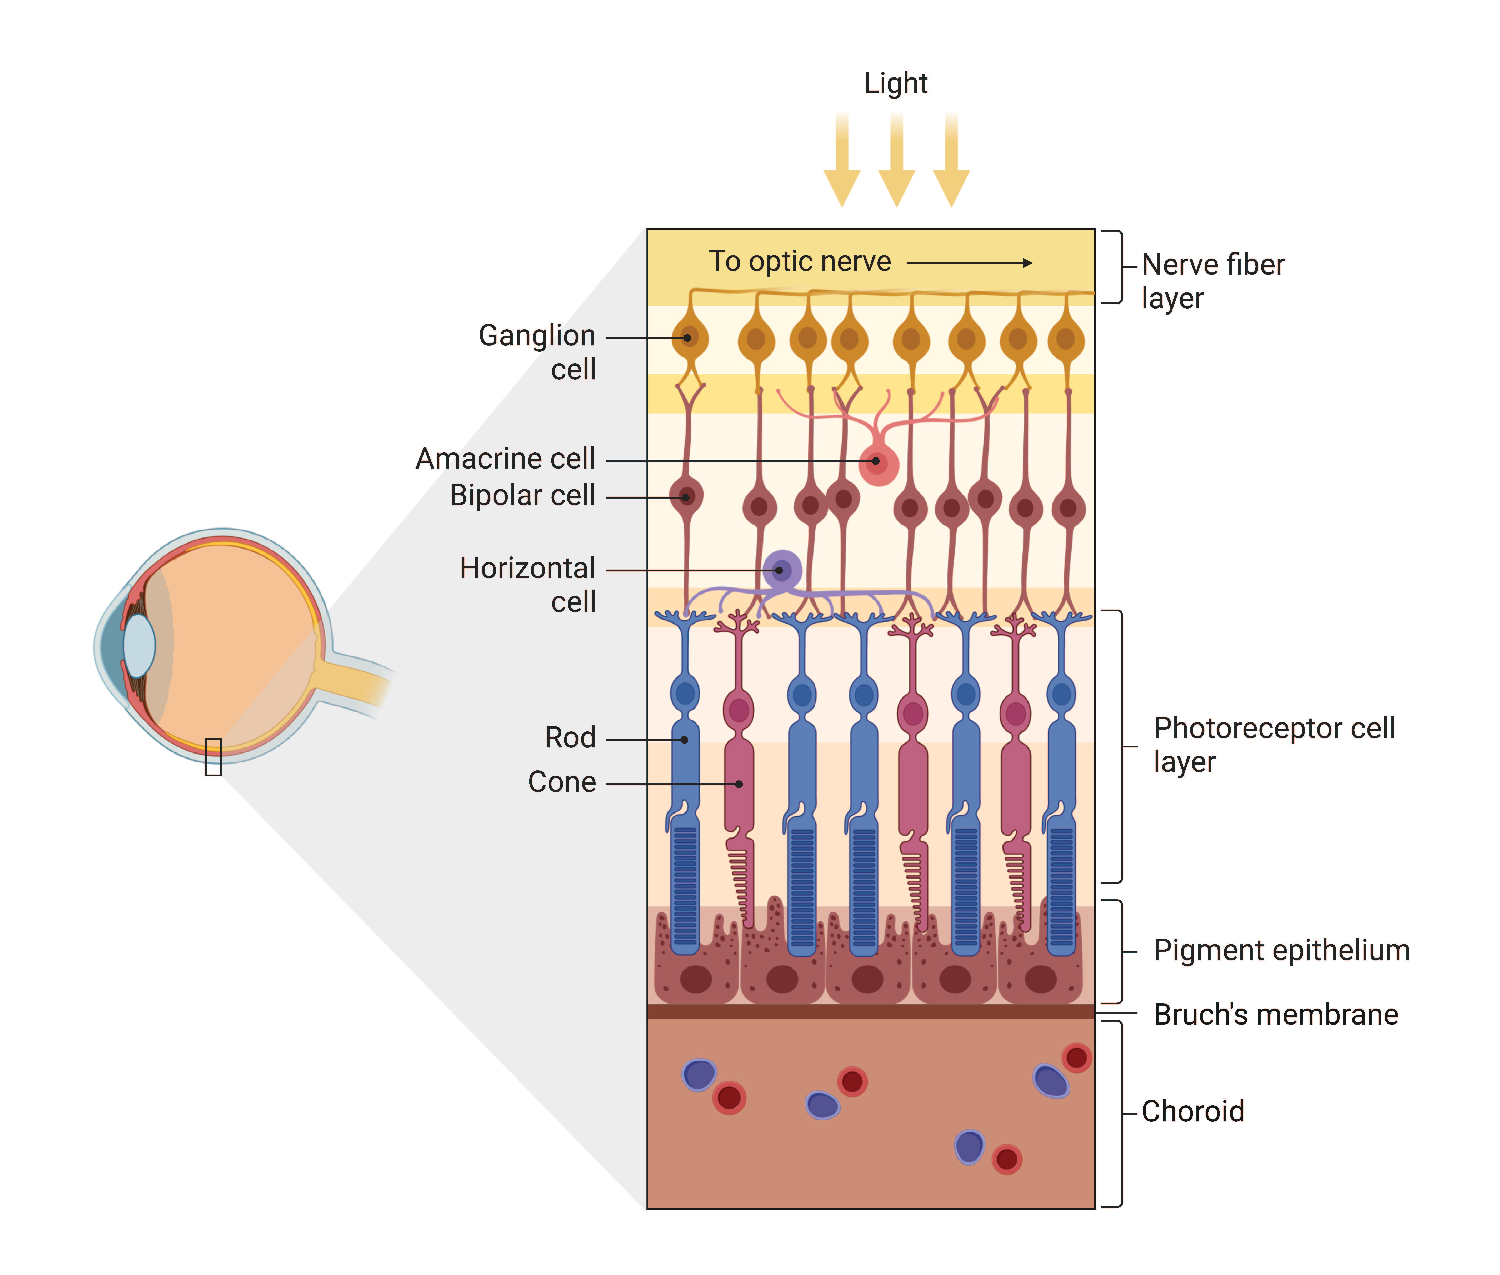
\includegraphics[width=\linewidth]{img/retina_anatomy.pdf}
    \caption{\textbf{Layered anatomy of the retina.} Adapted from \citet{schwartz1991principles}, 4th Edition, p. 436 and \citet{purves2019neurosciences}, 6th Edition, p. 239. "Created in BioRender. Beinhauer, D. (2025) https://BioRender.com/oy5qz9v".}
    \label{fig:retina_anatomy}
\end{figure}


\section{Lateral Geniculate Nucleus}
\label{sec:lgn}

The next stage in visual processing occurs in the \emph{lateral geniculate nucleus (LGN)}, located in the thalamus on each side of the brain. The LGN is a key structure responsible for the initial cortical-bound processing of visual signals. It serves as the primary termination site for most optic tract fibers (\citet{bear2020neuroscience}, 3rd Edition, p. 313). From there, the majority of visual information is relayed to the \emph{primary visual cortex (V1)} via the optic radiation. V1 is the principal cortical area involved in conscious visual perception (see Figure~\ref{fig:visual_system_pathway}).

Damage to any part of the visual pathway—from the retina to the LGN to the V1—can result in various forms of visual impairment or blindness (\citet{bear2020neuroscience}, 3rd Edition, p. 313). Because of the structured, topographic nature of this pathway, lesions can often be traced to specific anatomical locations.

Interestingly, while the LGN receives direct input from the retina, the majority of its synaptic input actually originates from the cortex, particularly from V1. Although the exact functional role of this feedback remains under investigation, it is widely believed to support signal modulation and attentional feedback (\citet{bear2020neuroscience}, 3rd Edition, p. 318).

Anatomically, the LGN is composed of six distinct layers, each organized to separately process input from one eye. These layers exhibit concentric receptive fields similar to those found in retinal ganglion cells (see Figure~\ref{fig:on_off_cells}). Importantly, the layers maintain \emph{retinotopic} organization (\citet{bear2020neuroscience}, 3rd Edition, p. 319--320), preserving the spatial layout of the visual field across neurons.

Functionally, the LGN is responsible for maintaining multiple parallel processing streams, with distinct pathways specialized for detecting motion, color, and fine spatial details. These properties make the LGN a fundamental stage for visual signal refinement and dynamic modulation, and also mark the beginning of feedback-dependent processing. For a more comprehensive description of LGN function and structure, refer to \citet{bear2020neuroscience} (3rd Edition, p. 315--320).

\section{Primary Visual Cortex}
\label{sec:v1}

The primary visual cortex (V1) is the first cortical area fully specialized for visual processing. It is located in the occipital lobe at the back of the brain. V1 is responsible for the initial cortical analysis of visual stimuli, including the encoding of orientation, size, motion, and color. Its outputs are split into two major processing streams: the parvocellular (P) stream, associated with form and color, and the magnocellular (M) stream, associated with motion and spatial information (\citet{bear2020neuroscience}, 3rd Edition, p. 330--332).

V1 is composed of six layers, conventionally labeled with Roman numerals (\citet{bear2020neuroscience}, 3rd Edition, p. 320). Input from the LGN is primarily directed to layer IV, which is further subdivided into layers IVA, IVB, IVC\textsubscript{\ensuremath{\alpha}}, and IVC\textsubscript{\ensuremath{\beta}}. This layer primarily processes monocular input. The output is then relayed to layers II and III (\citet{bear2020neuroscience}, 3rd Edition, p. 322), which are functionally similar and often grouped together as layer II/III. From this point onward, binocular integration becomes dominant. Outputs from these layers project to extrastriate areas such as V2 and V3, where higher-level visual processing occurs. Layers I, V, and VI are primarily involved in feedback and modulatory functions, with layers V and VI specifically contributing to recurrent processing from earlier visual stages (\citet{bear2020neuroscience}, 3rd Edition, p. 323).

Interlaminar connectivity is a key feature of V1, particularly within layer IV, where excitatory and inhibitory neurons form dense recurrent circuits that refine visual features. Inhibitory interneurons typically influence neurons within their own layers, while excitatory pyramidal neurons project across layers to support hierarchical processing (\citet{bear2020neuroscience}, 3rd Edition, p. 320--323).

V1 also exhibits \emph{retinotopy} (mentioned in Section~\ref{sec:lgn}), a topographic organization whereby neighboring neurons correspond to adjacent locations in the retina, LGN, and visual field. This mapping is not uniform—central regions of the visual field are represented with greater cortical magnification than peripheral regions.

\subsection{Receptive Field Properties of V1 Cells}
\label{subsec:receptive_field}

Neurons in V1 are organized into overlapping, interconnected functional maps, each tuned to specific features of visual stimuli. These include:

\begin{description}
    \item[Orientation selectivity:] Starting in layer IVC\textsubscript{\ensuremath{\alpha}} and IVC\textsubscript{\ensuremath{\beta}}, receptive fields become elongated, and neurons begin responding preferentially to stimuli of particular orientations. These preferences vary gradually across the cortical surface. Orientation selectivity gives rise to two classes of cells:
    \begin{description}
        \item[Simple cells:] These neurons are selective for both the orientation and position of a stimulus. Their receptive fields contain distinct ON and OFF regions, and their responses can be modeled as the sum of aligned LGN inputs.
        \item[Complex cells:] These neurons are orientation selective but respond across the entire receptive field, regardless of precise stimulus location. Their responses can be modeled as the pooled output of multiple simple cells.
    \end{description}
    See \citet{bear2020neuroscience} (3rd Edition, pp. 325--329) for further discussion.

    \item[Direction selectivity:] Some V1 neurons respond preferentially to motion in a specific direction, typically orthogonal to the orientation axis.

    \item[Binocularity:] While early layers (such as IV) are largely monocular, higher layers integrate signals from both eyes, allowing binocular perception and depth processing.

    \item[Other selectivities:] Additional V1 neurons are tuned for motion sensitivity, depth cues, feedback modulation, and color processing.
\end{description}

For a more comprehensive description of V1 function and structure, refer to \citet{bear2020neuroscience} (3rd Edition, p. 318--333).

The functional architecture and tuning properties of V1 lay the groundwork for computational modeling in visual neuroscience. By abstracting key principles such as orientation selectivity, hierarchical processing, and receptive field organization, researchers can build computational models that emulate early visual processing. These models not only shed light on underlying biological mechanisms but also provide a framework for testing how complex visual representations arise from structured cortical circuits.

\section{Extrastriate Visual Cortex}
\label{sec:extrastriate}

Beyond V1, visual processing continues in a network of extrastriate cortical regions that extract increasingly abstract features of the visual scene. These areas include V2, V3, V4, and MT (middle temporal area) (Figure~\ref{fig:early_vis_processing}), each contributing to distinct aspects of perception such as object recognition, motion tracking, and depth analysis. Damage to these regions does not typically result in complete blindness, but instead leads to specific deficits, such as achromatopsia (loss of color perception) or motion blindness (inability to perceive fluid motion), depending on the affected region. For a more comprehensive description of extrastriate cortical regions function and structure, refer to \citet{bear2020neuroscience} (3rd Edition, p. 333--337).